\section{Detailed technical assessments}\label{app:technical-details}

\subsection{Integrity under attack (DR1)}

We generated \TamperBase{} receipts from runs across all seven adapters and applied the mutations in Table~\ref{tab:tamper}. Of the cases the harness classifies as attacks, \TamperRejected{} of \TamperAttacks{} were rejected. Body edits failed signature verification whether the attacker kept the original signature, re-canonicalized correctly, or re-signed with an untrusted key under the legitimate key identifier. Non-canonical encodings were rejected as canonicalization mismatches. A valid receipt presented a second time is accepted: the verifier keeps no replay cache. Audience, nonce, and a caller-supplied version floor are checked only when requested. \code{expiresAt}, when the issuer set it, is enforced on every verification. Presenting the same receipt again is therefore not, by itself, a failed verification. What the verifier did not check is reported as structured advisories, each with a code and a severity. A warning means the receipt is bound to an audience or a nonce that the caller did not check. An information advisory means the receipt carries no audience, nonce, or expiry, or sits below the current schema version. The command-line verifier always prints warnings and prints information lines unless \code{--quiet} is set. Figure~\ref{fig:rw-tamper-heat} applies comparable mutation classes to the other record systems of Section~\ref{sec:realworld}.

Chain checks are separate from the single-receipt \code{VerifyErrorKind} taxonomy. \code{verifyChain} reports its own error kinds (\code{VerifyChainErrorKind}): an invalid link, no root, multiple roots, an orphan link, a run-identifier mismatch, a duplicate content identifier, a count mismatch, or a root mismatch. Reordering the receipt array is not an error, because the verifier follows parent links rather than array position. Dropping a middle link, splicing a foreign link, or replacing the root fails that check. Truncating the tail of an open chain does not. The result is success plus a tail-truncation warning unless the caller passes \code{expectedCount}. A chain whose root declares \code{chainClosure} fails with a count mismatch when a leaf or the closing receipt is missing, with no expected count, and a malformed closing receipt fails as an invalid link. \code{requireClosure} turns a missing closure declaration into a failure, and \code{partial} accepts a disclosed subset only when the closing receipt is present and lists every presented receipt, and warns when some listed members were not presented. Table~\ref{tab:v16} records these checks together with the advisories, crew receipts, and signer-failure modes. \VerifierChecksPassed{} of \VerifierChecks{} checks passed. Two of them run the released 1.6.0 verifier on a closed crew chain and confirm that it accepts the chain without enforcing closure.

\subsection{Verifiable retained evidence (DR2)}

For each of the seven adapters we recorded runs against provider-shaped fixtures, wrote the receipt and content-addressed artifacts to disk, reloaded them, verified the receipt, materialized a replay envelope, replayed offline, and recomputed the output hash. \ReplayVerified{} of \ReplayRuns{} runs verified, and \ReplayHash{} reproduced the signed output hash. Re-executing each run against the same fixture matched in \ReplayLive{} cases, and a one-character change to a recorded output was detected in \ReplayAltered{} cases (Table~\ref{tab:replay}). These results show that the record is internally consistent. Offline replay does not call a model: \code{replayOffline} returns the outputs the caller supplies, and the check is that they hash to the signed output hash. The result is therefore a signed output binding, which other signed record systems also provide (Table~\ref{tab:rw-matrix}). On the hosted rerun, every replayed receipt verified and a one-character edit was detected, and the signed output hash matched the kept answer except on trials that stored an empty answer after a provider failure (Figure~\ref{fig:rw-replay}). That mismatch is not a signature or chain failure. The check does not show that a live model would reproduce its output, and repeated live calls often returned different answers (Figure~\ref{fig:rw-drift}). Those historical bindings covered input artifacts and outputs only, with no task commitment. Current optional v1.4 fields extend that boundary, but do not turn the historical replay counts into tests of task or policy binding. In a crew chain, the crew-start receipt hashes the nested agent tree (\code{\{kind: "crew-start", agents: \{id, children\}\}}), each completion receipt hashes its agent's output, and the crew-close receipt hashes its member list.

\subsection{Inspectable execution and control outcomes (DR3)}\label{app:policy-details}

\paragraph{Routing.} Using a synthetic catalog of 40 model capabilities and \RouteRequests{} random requests with random policies, repeated decisions were identical at rate \RouteIdentical{}. An independently implemented oracle found \RouteViolations{} selected routes that violated provider allow or deny lists, privacy class, logging, latency, or image-modality constraints, and \RouteFalseNo{} cases in which the router reported no route although a feasible candidate existed. Reordering the catalog changed the selected model at a same-selection rate of \RoutePermSame{}. Catalog position is not part of the score, and ties break on provider and model identifiers. The receipt signs the selected route and the requested and observed model. In the historical experiment it did not sign the policy. Current task and policy hashes permit expected-content checks, while the policy itself, candidate list, scores, and catalog version still require separately retained records to recompute the decision.

\paragraph{Personal-data invariant.} The following rules and scores describe the detector revisions used by the historical experiments. They cover four types, and each rule trades recall for precision in a stated way. Email addresses match as written. A dashed United States social security number (SSN) matches as written. Spaced and undashed nine-digit forms match only when an SSN cue such as \code{ssn}, \code{ss\#}, or \code{social security} is the nearest word. Separated United States phone numbers match as written. A plain ten-digit run matches only when it is a valid North American number and the nearest word is a phone cue (\code{phone}, \code{tel}, \code{call}, \code{mobile}, \code{cell}, or \code{fax}) or a \code{+1} or \code{1-} trunk prefix precedes it. A payment card number is any Luhn-valid run of 13 to 19 digits, except runs that start with 0 or 1 and 13-digit runs that start with 978 or 979, which are ISBN-13 numbers. An SSN, phone, or card match is suppressed when an identifier label (\code{order}, \code{ord}, \code{invoice}, \code{inv}, \code{sku}, \code{ref}, \code{po}, \code{isbn}, \code{pn}, or \code{txn}) is the nearest token on the same line, joined to the number only by whitespace or by \code{:}, \code{\#}, \code{=}, \code{no.}, \code{number}, or \code{is}, unless the number is a phone number with a trunk prefix. Labels do not suppress email addresses. Words such as customer, account, and ticket are not labels. The trade-offs follow from these rules. A real SSN written as \code{order 123-45-6789} is not flagged. A bare nine- or ten-digit number without a type cue is not flagged, whether or not it is personal data. About one in ten random digit strings passes the Luhn check, so a text that lists $k$ numeric identifiers of 13 to 19 digits is flagged as holding a card with probability near $1-0.9^{k}$. The detectors see only strings, so a value stored under a key such as \code{ssn} is judged by its digits alone.

We built a labeled set of synthetic strings, 100 per label. In-scope positives cover each form the detectors claim, support-ticket text in which a number follows words such as customer, account holder, or patient ID, CSV and markdown rows, and card numbers from several networks. Out-of-scope personal data are names with addresses, international bank account numbers, United Kingdom phone numbers, IP addresses, dates of birth, and spelled-out email addresses. Negatives include order identifiers and stock-keeping units shaped like SSNs or phone numbers, 16-digit references, ISBN-13 numbers, and uncued numbers such as timestamps, byte counts, and bank routing numbers. On in-scope types plus all negatives, \code{noPII} reached precision \PiiInPrecision{} and recall \PiiInRecall{} (\(n=\PiiInN\), false positives \PiiInFp{}, false negatives \PiiInFn{}). The false negatives come from forms the rules leave out by design, such as a plain ten-digit number after ``call the customer at'' and an undashed SSN in a CSV row with no SSN cue. The \PiiNewNegN{} uncued numeric negatives produced \PiiNewNegFp{} false positives. Counting every personal-data label, including types the detectors do not claim, precision was \PiiAllPrecision{} and recall \PiiAllRecall{} (Table~\ref{tab:policy}, Figure~\ref{fig:pii}). The cases were chosen with the rules in view, and the identifier-shaped negatives carry the labels the rules key on, so these figures show that the rules behave as specified. They are not prevalence-weighted estimates and not estimates of precision on real text. On public datasets, SSN and phone precision and recall were far lower, because passport numbers and other identifiers share the same digit shapes (Section~\ref{sec:realworld}, Figure~\ref{fig:rw-pii}, Tables~\ref{tab:rw-pii-ai4} and~\ref{tab:rw-pii-gretel}, Figures~\ref{fig:rw-pii-f1} and~\ref{fig:rw-pii-latency}). Those public-data rows were measured with the rules at commit \texttt{a8cc091}, which differ from the rules above as Section~\ref{sec:realworld} describes.

\paragraph{Citation invariant.} The \code{mustCite} invariant checks that an output cites a named artifact. By default it reads only structured lists: a top-level \code{citations} or \code{evidence} list whose string entries, or whose objects' \code{source} field, name the artifact. Matching is case-sensitive unless case folding is requested, and other object keys can be named. If the top-level list is missing or omits the artifact, nested \code{citations} and \code{evidence} lists are searched, unless the contract declares a path. The default never reads prose. Three options extend it, and each is added to the contract only when set, so the hash of an existing contract does not change. With \code{inline}, a bracketed or parenthesized group in the prose whose content, or one comma- or semicolon-separated part of it, equals the artifact name also counts; it does not override a non-empty structured list that omits the artifact. With \code{rejectUncited}, a matching list entry is rejected when the prose contains citation-like square brackets, such as \code{[1]}, \code{[1-3]}, or \code{[Smith 1999]}, and none of them resolves to the artifact. Links, footnote markers, and code are not treated as citations. \code{textPath} limits these prose checks to one field. The invariant agreed with the labels in \MustCiteAgree{} of \MustCiteCases{} constructed cases: \MustCiteDefaultAgree{} of \MustCiteDefaultCases{} for the default and \MustCiteOptInAgree{} of \MustCiteOptInCases{} for the options. The cases include numeric markers, links, and path-scoped outputs, and they were also chosen with the implementation in view. ASQA long answers are prose without citation lists, so the default accepts a gold title in none of them. The ASQA count in Section~\ref{sec:realworld} was measured at commit \texttt{a8cc091}, where an inline marker containing the name counted by default. The check is syntactic. It does not judge whether the cited artifact supports the claim \citep{lewis2020rag}.

\begin{figure}[t]
\centering
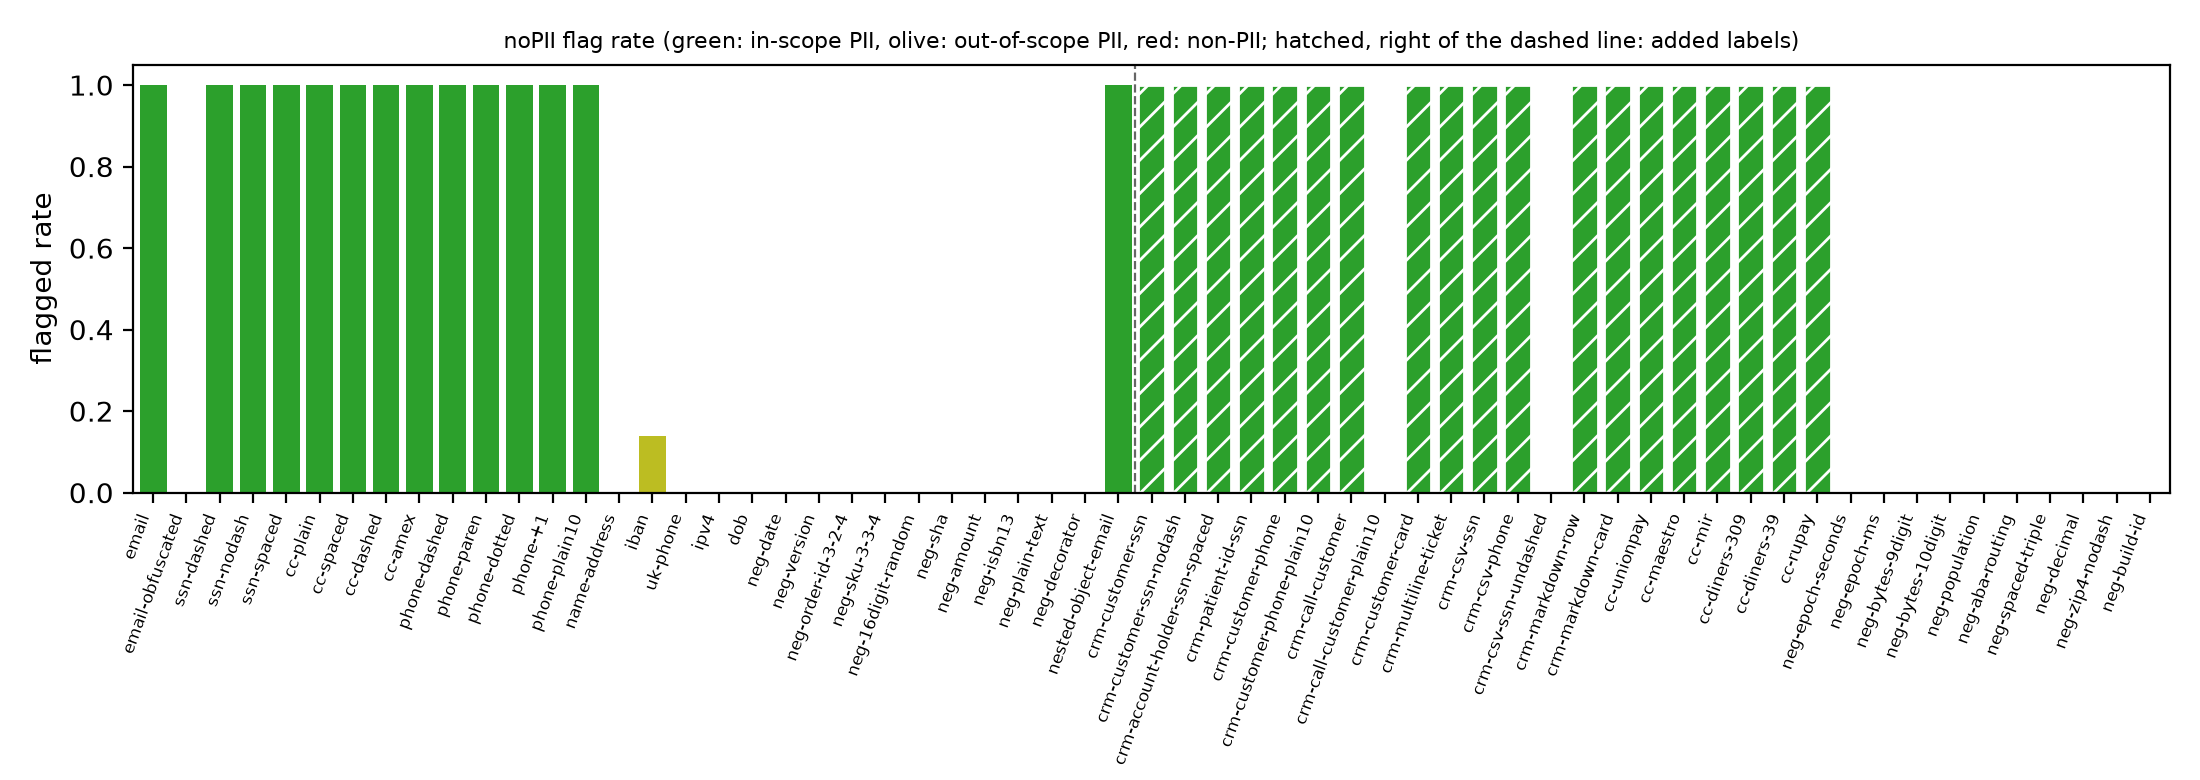
\includegraphics[width=\textwidth]{Fig4.png}
\caption{Share of samples flagged by the \code{noPII} invariant, by label. Green: in-scope personal data. Olive: out-of-scope personal data. Red: non-personal data. Plotted from \code{eval/results/policy.json}}
\label{fig:pii}
\end{figure}

\subsection{Minimized disclosure (DR4)}\label{app:disclosure-details}

We placed marker secrets in the task, an input artifact, the provider credential, and the model output, then scanned the decoded signed payload, with and without a \code{noPII} invariant. Marker hits in signed bytes were \LeakHits{} of \LeakRows{} rows (Table~\ref{tab:policy} does not repeat the per-adapter log; the raw rows are in \code{eval/results/policy.json}). Receipts carry hashes of the input artifacts and the output. In that historical recording, neither the task text nor the credential appeared in the signed bytes, in clear or as a hash. Current receipts add an unsalted task digest and may hash request bodies containing sensitive content; credentials in transport headers are outside that digest. When the invariant fires, the in-process tripwire result still includes the matched substring so the caller can act on it. The value that is signed is a detector name, a length, and a mask, so the signed bytes hold the masked form that the redaction manifest describes. The scan checks for the marker strings themselves. It does not test whether a hash can be inverted: a low-entropy input or output, such as an SSN or a yes/no answer, can be confirmed from its unsalted hash by dictionary search (Section~\ref{sec:requirements}, DP4). Among the record systems compared in Section~\ref{sec:realworld}, Figure~\ref{fig:rw-bytes} shows which kept the plaintext transcript and which kept only digests or ciphertext when wrapping the same recorded request and response bytes.

\subsection{Controlled latency and chain distributions}

\begin{figure}[t]
\centering
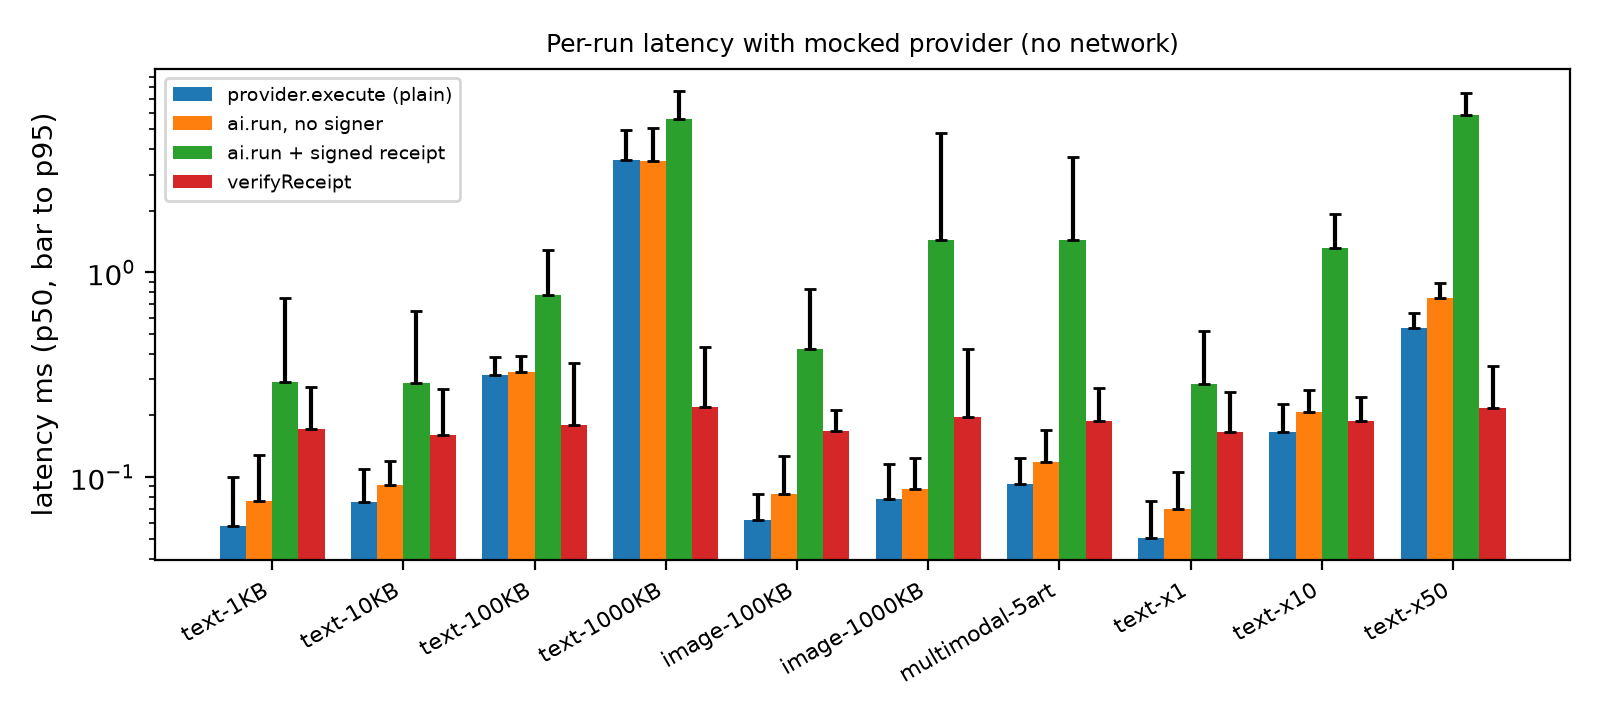
\includegraphics[width=\textwidth]{Fig2.png}
\caption{Per-run latency with a mocked provider across input configurations (log scale; bars show the median, whiskers extend to the 95th percentile)}
\label{fig:overhead}
\end{figure}

\begin{figure}[t]
\centering
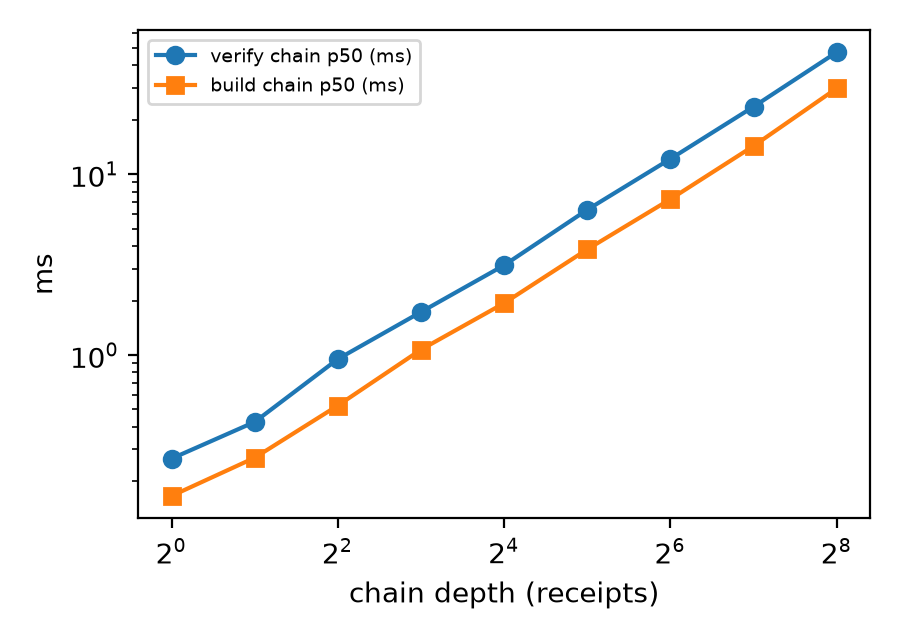
\includegraphics[width=0.72\textwidth]{Fig3.png}
\caption{Build and verification time of linked receipt chains by depth}
\label{fig:chain}
\end{figure}

\FloatBarrier
